\documentclass[11pt,a4paper,oneside, openright]{article}
\usepackage{graphicx}
\usepackage[british]{babel}
\usepackage[utf8]{inputenc}
\usepackage{mathtools}
\usepackage{setspace}
\usepackage{verbatim}
\usepackage[htt]{hyphenat}
\usepackage{url}
\usepackage{amsmath}
\usepackage{placeins}


\begin{document}
{\setstretch{1.0}
  \begin{titlepage}
  	\centering
  	
\includegraphics[width=6cm]{images/unipi.eps}\par
  	\vspace{1.5cm}
  	{\huge\textsc{Performance evaluation of a CRAN system}\par}
  	\vspace{2cm}
  	Gerardo \textsc{Alvaro}\par
  	Francesco \textsc{Barbarulo}\par
    Francesco \textsc{Fornaini}

  	\vfill

    % Bottom of the page
  	{\large 2018-2019\par}
  \end{titlepage}
}


\tableofcontents

\newpage

\section{Introduction}
\label{sec:introduction}

The system examined is a simplified version of an architecture presented for future cellular networks, called Cloud-RAN (CRAN).

\subsection{Description of the system}
 At the center of this system there is a central processing unit (BBU), which is responsible for forwarding the packets received from an Application Server (AS) to one of the N remote radios (RRH) connected to it. Each RRH serves a single cell, and each packet generated by the AS has one of these cells as destination, taken uniformly from the available ones. Each data packet has a size $s$ and a new one is generated every $t$ seconds. The BBU has an interface to each of the RRHs and communicates with only one of them at a time, at a speed of X bytes/s. If the BBU interface with the RRHs is busy, the data packets are queued and served using the FIFO policy.

When the BBU receives a packet from the AS, it can operate in two different ways:
\begin{itemize}
	\item[A)]It retransmits directly the packet to the RRH which serves the destination cell N;
	\item[B)]The BBU compresses the packet, reducing its size by C\% and retransmits it to the proper RRH. Once arrived at the RRH, the packet is decompressed. Such operation takes S seconds, where S is given by $ S = C \cdot 50ms $. Only one packet can be decompressed at a time. If the decompressing process is busy, the incoming data packets are queued and served using a FIFO policy.
\end{itemize}

Packet size and interarrivals are random variables described as:
\begin{itemize}
	\item exponential distribution of $t$;
	\item exponential and lognormal distribution of $s$.
\end{itemize}

\subsection{Objectives and performance indexes}
???
The objective of the study is to determine if and under which conditions it is better to perform packet compression or not.
For a correct evaluation of the system will be taken as reference the mean end-to-end delay of packets.

\newpage

\section{Model}
The model, according to the queueing theory, is the following:
\begin{figure}[h]
	\centering
	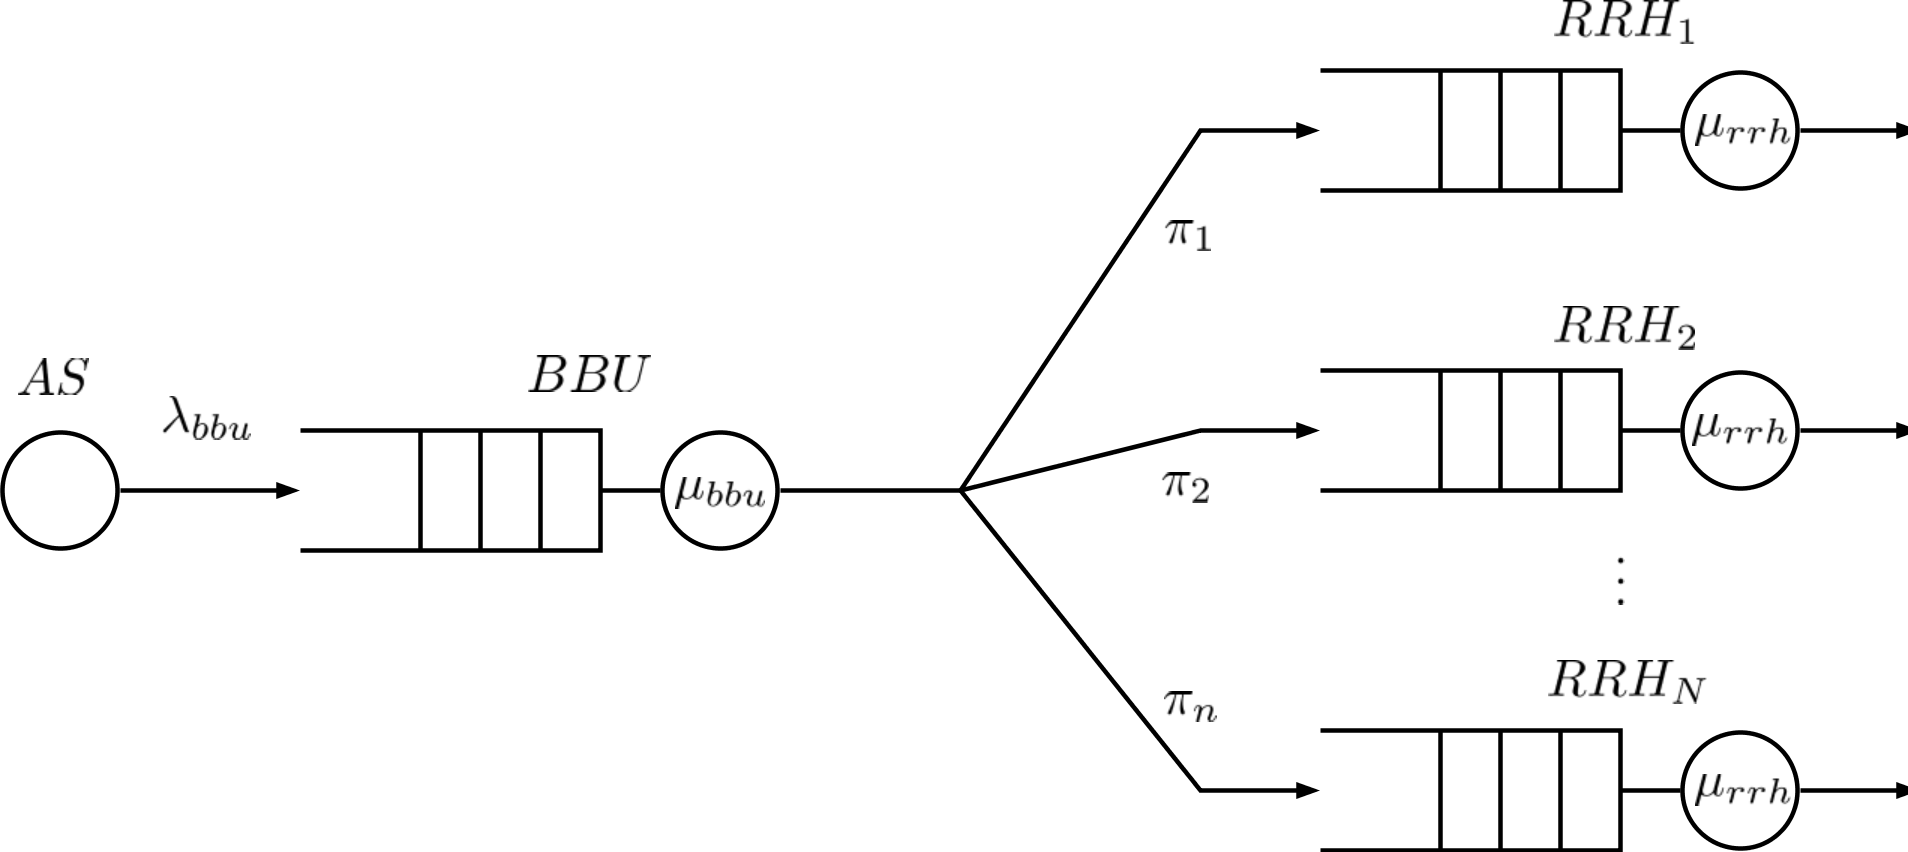
\includegraphics[width=0.9\textwidth]{images/model}
	\caption{Queueing network model}
	\label{fig:model}
\end{figure}

We make some semplifications which do not affect the final results:
\begin{itemize}
    \item Propagation times ($ T_{prop} $) are negligible;
    \item BBU switching time (time needed to change the output gate) is negligible;
    \item In case B, the compression time on BBU is negligible;
    \item Packets are not corrupted;
    \item No packet loss at the buffers (infinite buffers).
\end{itemize}

With these assumptions, we can compute the end-to-end delay as following:

$$ T_{delay} =  T_{waiting\_bbu} + T_{transmission} + T_{waiting\_rrh} + T_{decompression} $$

where 

$$ T_{transmission} = \frac{1}{\mu_{bbu}} = \frac{s}{X} $$

and

$$ T_{decompression} = \frac{1}{\mu_{rrh}} = C \cdot 50ms $$

\subsection{Validation}
The simulator has been validated through a comparison with a queueing theory model of the system.

The system has been modelled as an Open Jackson Network because all the hypotheses are verified since external arrivals are poissonian and routing probabilities are state-independent because they are uniform as specified in the requirements.

\subsubsection{Stability conditions}
In order to compute the stabilty conditions we have to distinguish between the two cases.

In case A we have to respect only one condition regarding the BBU. Indeed, on the RRHs we will never have queues because when the packet arrives it is immediately consumed.
Hence, the stability condition is the following:

$$ \lambda_{bbu} < \mu_{bbu}, \quad \lambda_{bbu} = \frac{1}{t}, \quad \mu_{bbu} = \frac{X}{s}$$

\begin{equation} \label{eq:rho-bbu}
\rho_{bbu} = \frac{\lambda_{bbu}}{\mu_{bbu}} = \frac{s}{t \cdot X} < 1
\end{equation}

Note that $s$ represents the number of bytes that the BBU has to transmit. From now on we will consider:
$$s = s\cdot(1-\frac{C}{100})$$

In case B we have also to take in account the stability condition on the RRHs because now the RRH service time is not null and depends on the compression percentage. 

We have to guarantee that the arrival rate of the RRHs is poissonian. If we consider just one RRH, the model can be seen as a tandem QN which respects Burke's theorem. Hence, the arrivals at the RRH are a Poisson process with rate $ \lambda_{bbu} $ regardless of the BBU service rate, that, in our simulations, will be both exponential and lognormal. 
Obviously, this reasoning can be extended in a system with more than one RRH, where the arrival rate will depend on the number of remote radios as follows:

$$ \lambda_{rrh} = \lambda_{bbu} \cdot \pi = \frac{1}{t \cdot N} $$

$$ \mu_{rrh} = \frac{1}{C \cdot k}, \quad k = 50ms $$

\begin{equation} \label{eq:rho-rrh}
\rho_{rrh} = \frac{\lambda_{rrh}}{\mu_{rrh}} = \frac{C \cdot k}{t \cdot N} < 1
\end{equation}
% questo è ok in condizione di stabilità, ma queste SONO le condizioni di stabilità

Hence, using the result obtained in \eqref{eq:rho-bbu}, the final stability condition for case B is:

$$ \begin{cases} \rho_{bbu} = \frac{s}{t \cdot X} < 1 \\ \\ \rho_{rrh} = \frac{C \cdot k}{t \cdot N} < 1 \end{cases} $$

with steady state probability, either on BBU and RRHs, equal to:

$$ p_{n} = \rho^n \cdot (1 - \rho) $$

Note that the steady state probability on each RRH and on the BBU is equal to an M/M/1.

% At the steady state, by Burke's theorem, the departure process at the BBU, which is an M/M/1, is a Poisson process with a rate $ \lambda_{bbu} $.

\subsection{Statistics for validation}
In order to validate our model we have used the following perfomance indexes taken from the queueing theory:

$$ E[N_{bbu}] = \frac{\rho_{bbu}}{1 - \rho_{bbu}} = \frac{s}{X \cdot t - s}$$

$$ E[R_{bbu}] = \frac{E[N_{bbu}]}{\lambda_{bbu}} $$

$$ E[N_{rrh}] = \frac{\rho_{rrh}}{1 - \rho_{rrh}} = \frac{C \cdot k}{t \cdot N - C \cdot k}$$

$$ E[R_{rrh}] = \frac{E[N_{rrh}]}{\lambda_{rrh}} $$
%?
The successful comparison between these equations and the simulator results assure us that we are working on a correct model for our system.
%?

\section{Simulator implementation}
The simulator consists of four modules as shown in Figure~\ref{fig:simulator}:
\begin{itemize}
  \item \texttt{As}: it creates/produces a packet flow according to the interarrival time sending them to the BBU;
  \item \texttt{Bbu}: it forwards the packets received from the AS to the RRH, compressed if it has to;
  \item \texttt{Rrh}: it decompresses the packet, if it was compressed, and sends it to the collector for the delay statistics;
  \item \texttt{Collector}: it handles of the delay statistics.
\end{itemize}

\begin{figure}[h]
    \centering
    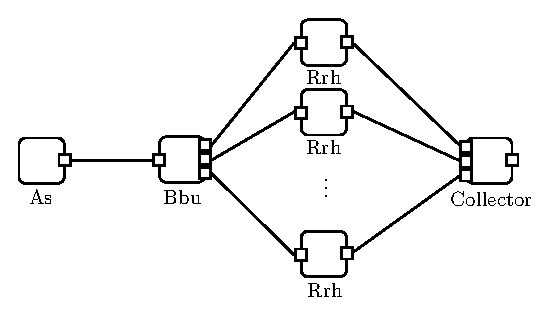
\includegraphics[width=0.9\textwidth]{images/simulator}
    \caption{Simulator architecture}
    \label{fig:simulator}
\end{figure}

\subsection{Application Server (AS)}
The As module has to perform cyclically the following operations:
\begin{itemize}
    \item[1.] it creates a new packet with the \texttt{id}, the packet size \texttt{s} taken either from an exponential distribution or a lognormal one, the destination taken from an uniform distribution, the creation time \texttt{created\_at};
    \item[2.] it sends the packet to the BBU;
    \item[3.] it waits according to the interarrival time \texttt{t} taken from an exponential distribution.
\end{itemize}

\subsection{Baseband Unit (BBU)}
When the Bbu module receives a packet from the AS it has to do the following actions:
\begin{itemize}
    \item[1.] if it is idle, it processes the packet immediately, otherwise the packet will be queued and served using a FIFO policy;
    \item[2.] it processes the packet deciding whether the packet must be compressed or not and transmitting it to the proper RRH;
    \item[3.] if there are any other packets in the queue, the first of them is pulled off from the buffer and served, otherwise it waits for the next packet.
\end{itemize}

\subsection{Remote radio (RRH)}
When one of the N RRHs receives a packet from the BBU, it acts as follow:
\begin{itemize}
    \item[1.] if it is idle, it processes the packet immediately, otherwise the packet will be queued and served using a FIFO policy;
    \item[2.] it processes the packet deciding whether the packet must be decompressed or not and transmitting it to the Collector;
    \item[3.] if there are any other packets in the queue, the first of them is pulled off from the buffer and served, otherwise it waits for the next packet.
\end{itemize}


\subsection{Collector}
The Collector module (virtually) collects all the packets coming from the RRHs and deals with the end-to-end delay statistics.



\section{Verification}
The simulator has been verified in order to check for memory leaks and bugs.
For the first ones we have used Valgrind tool, whereas, for bugs, we have done some simulations with known results.

We have set proper values, for both \texttt{warmup-time} and \texttt{simulation-time-limit}, according to some simulation results.
\begin{figure}[h]
	\centering
	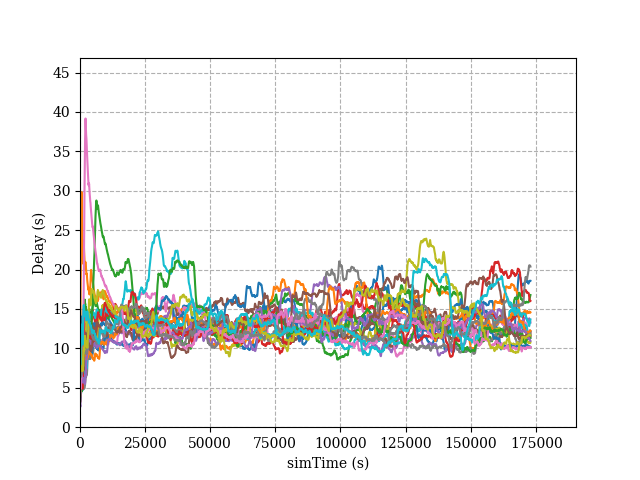
\includegraphics[width=0.9\textwidth]{images/warm-up}
	\caption{Warm-up study}
	\label{fig:warm-up-study}
\end{figure}

We have estimated the \texttt{warmup-time} applying the sliding window average (windowSize = 10000) to the mean end-to-end delay values obtained from 20 independent repetitions of our highest value of $ \rho_{bbu} $ (0.9). The same reasoning will be applied to the next simulations.

In Figure~\ref{fig:warm-up-study} it is shown that a good value for \texttt{warmup-time} is around 50000 seconds, where the initial transient is over and the steady state is reached. 

The value for the \texttt{simulation-time-limit} has been chosen in order to have enough results for statistics (i.e. 2 days of simulation time).

\section{Experiments}
We will analyze separately the two cases described in Section~\ref{sec:introduction} either with exponential and lognormal distribution, the latter only for the packet size.
We will take in account scenarios with at least 2 remote radios, because a system with only one remote radio is not interesting to analyze. Futhermore, the number of RRH has to verify the stability condition computed in \eqref{eq:rho-rrh}. For each case we have done 20 different repetitions for every single scenario.

\subsection{Case A - Transmission without compression}
In this case the end-to-end delay could depend on two factors:
\begin{itemize}
	\item \texttt{X}, chosen such as $ \rho_{bbu} $, computed as in \eqref{eq:rho-bbu}, will assume values from 0.1 to 0.9 increased by 0.1;
	\item \texttt{N}, with prefixed values of 2, 5, 10.
\end{itemize}
\subsubsection{Exponential}
Since the exponential distribution does not provide a variance control, the packet size \texttt{s}, extracted by the AS, could assume both small and large values.

\begin{figure}[h]
	\centering
	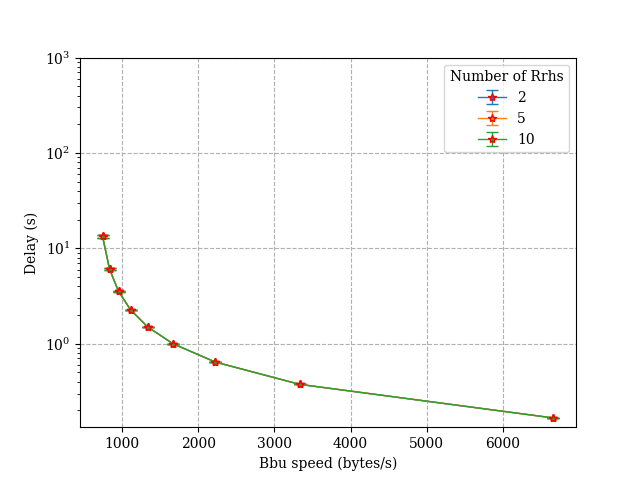
\includegraphics[width=0.9\textwidth]{images/case-a-exp}
	\caption{Case A - Exponential distribution}
	\label{fig:exp-a}
\end{figure}

In Figure~\ref{fig:exp-a}, as we expected, we can see that the end-to-end delay does not depend on the number of remote radios \texttt{N} because on the RRH the service time is null, so there will be no queues and the packets will be forwarded to the cells immediately.

In fact, the three different plots (2, 5 and 10 RRHs) overlap perfectly.
Hence, the only factor that allows to minimize the end-to-end delay is the BBU transmission speed \texttt{X}.


%\begin{align}
%E[R] &= E[R_{bbu}] \notag \\
%&= E[W_{bbu}] + \frac{1}{\mu_{bbu}} \notag \\
%\end{align}
\subsubsection{Lognormal}
In the lognormal scenario, the probability to have packet size values greater than the mean value is higher with respect to the exponential distribution. For this reason the end-to-end delay (shown in Figure~\ref{fig:log-a}) tends to be higher than the previous analysis as \texttt{X} decreases.

Furthermore, we can notice that the confidence interval for lower values of \texttt{X} ($\rho \simeq 1$) is wider than the exponential one. This is due to the fact that the system is sensitive to an unlucky stream of packet whose size is greater than the mean size value.

\begin{figure}[h]
	\centering
	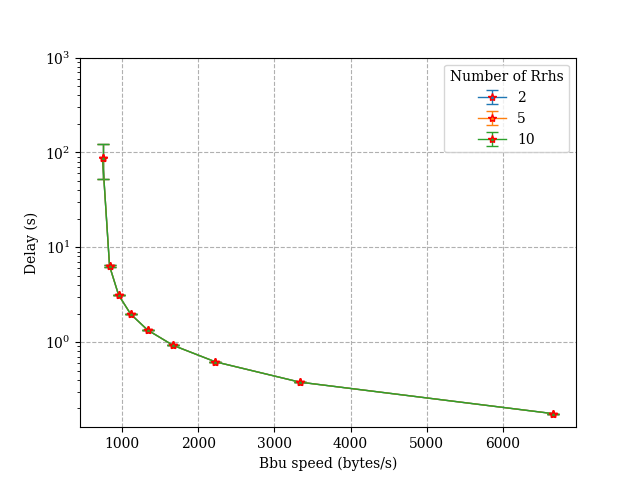
\includegraphics[width=0.9\textwidth]{images/case-a-logn}
	\caption{Case A - Lognormal distribution}
	\label{fig:log-a}
\end{figure}

Of course, also in this case, the only meaningful scalable factor is the BBU transmission speed.
\bigbreak
\noindent The data for both distributions have been tested with a level of confidence interval of 99\%. 

\subsection{Case B - Transmission with compression}
In addition to the factors of case A, now we have a further factor to take in account: the compression percentage. Hence, the set of factors becomes:

\begin{itemize}
	\item \texttt{X}, that will assume the same values of case A, but we have to consider that now $ \rho_{bbu} $ depends on the compression percentage because of the smaller number of bytes transmitted. We have chosen these values for the sake of a correct comparison between the two cases.
	\item \texttt{N}, with values ranging from 2 to 50.
	\item \texttt{C}, with values ranging from 10 to 90.
\end{itemize}

\subsubsection{Exponential}
According to inequality expressed in \eqref{eq:rho-rrh}, $ \rho_{rrh} $ does not depend on \texttt{X}, thus, we can fix the BBU speed (i.e. 1000 bytes/s) and compare the results obtained from the variations of \texttt{N} and \texttt{C}. Futhermore, we need at least 4 RRHs in order to be able to compress up to 90\% keeping $ \rho_{rrh} < 1$. For this reason, we will not show the trend of the waiting time in a system with 2 or 3 RRHs because it would not respect the stability condition.

In Figure~\ref{fig:c-vs-waiting}, we take in account only the waiting time on the RRHs because the service time is constant at same values of compression \texttt{C} which would cause only a linear upward translation of the graph.

\begin{figure}[h]
	\centering
	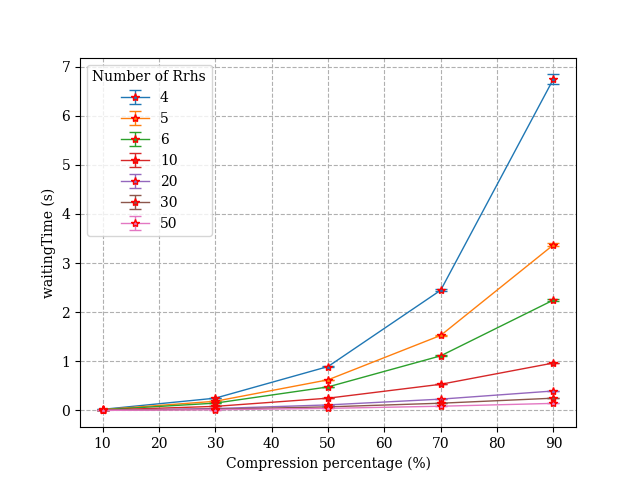
\includegraphics[width=0.9\textwidth]{images/c-vs-waiting}
	\caption{Waiting time trend in relation to \texttt{C} and \texttt{N}}
	\label{fig:c-vs-waiting}
\end{figure}

As the number of RRHs increases, the waiting time tends to be constant around zero becoming independent from the compression percentage.


Hence, for what we noticed in the above consideration, we can fix the number of RRH to an high value (i.e. 20) in order to have a short waiting time on the RRHs, and see how the end-to-end delay varies as BBU speed and compression percentage change.

\begin{figure}[h]
	\centering
	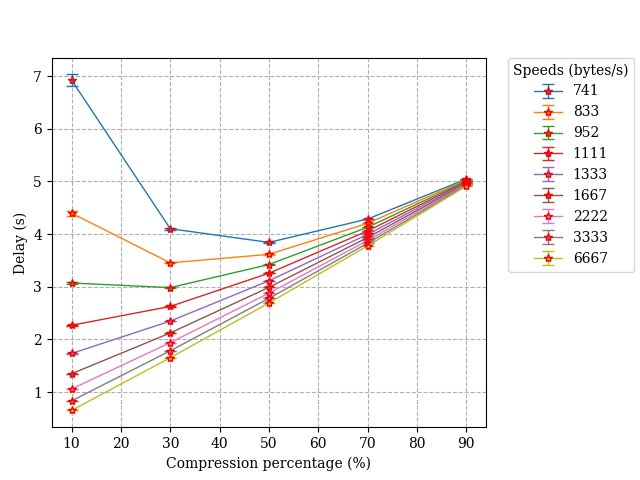
\includegraphics[width=0.9\textwidth]{images/c-vs-delay}
	\caption{End-to-end delay trend in relation to \texttt{C} and \texttt{X}}
	\label{fig:c-vs-delay}
\end{figure}

In Figure~\ref{fig:c-vs-delay} it is shown that as the compression percentage increases, the end-to-end delay tends to become flat, making the BBU speed less significant. Furthermore, also in this experiment where waiting times on the RRHs are minimal, for none of the BBU speeds taken into consideration we have an advantage in setting the compression percentage over 50\%. For this reasoning from now on we will consider the compression percentage with values ranging from 10 to 50 and this allows us to comply the inequality $ \rho_{rrh} < 1$ even for 2 and 3 RRHs.


In the final analysis let's look at the trend of the delay when all three factors vary as follows:

\begin{itemize}
	\item \texttt{X}, that will assume the following values: 741, 833, 952; considering that for all the other values there is never any advantage in increasing the compression percentage.
	\item \texttt{N}, with values ranging from 2 to 20.
	\item \texttt{C}, with values ranging from 10 to 50.
\end{itemize}


\end{document}